\section{Hormiga de Langton}
\subsection{Introducción}
La hormiga de Langton es un autómata celular desarrollado por Chris Langton en 1968, Langton se inspiro en la bioquímica, exploró la posibilidad de implementar la lógica molecular del estado viviente generando así una bioquimica artificial basada en la interacción entre moléculas artificiales. Langton dijo que el comportamiento global de una sociedad es un fenómeno emergente que surge de todas las interacciones locales de sus miembros. 

El comportamiento complejo puede surgir de la interacción de las partes muy simples. Por lo que utilizo una colonia de hormigas como modelo para una forma variante de un autómata celular, en donde cada célula puede cambiar de estado, en virtud de los estados de las otras células. \cite{LANGTON}

\begin{figure}[H]
\begin{center}
 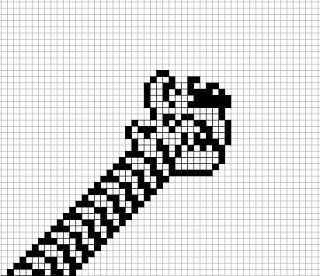
\includegraphics[width=8cm, height=6cm]{img/ant.jpg}
 % ant.jpg: 320x276 px, 72dpi, 11.29x9.74 cm, bb=0 0 320 276
 \caption{Ejemplo de una hormiga de Langton}
 \label{fig:ant}
\end{center}
\end{figure}

Las hormigas del modelo clásico se mueven en un entorno que consta de células en donde cada una de estas células se encuentra en uno de los dos posibles estados (viva o muerta, 0 o 1), la hormiga viaja en linea recta en el espacio siguiendo las siguientes reglas:
\begin{description}
 \item Si se encuentra con una célula muerta, hace un giro a la derecha y sale de la célula invirtiendo el estado de la misma.
 \item Si se encuentra con una célula viva, gira a la izquierda y sale de la célula invirtiendo su estado.
\end{description}

De esta forma la hormiga deja un "rastro" a medida que se mueve.

\subsection{Práctica a realizar}
En esta práctica se trabajaron dos versiones diferentes de la hormiga de Langton, la primera que es la implementación clásica de este autómata celular y la segunda versión en la cual se cuenta con tres tipos de hormigas y de restricciones que modifican el comportamiento del autómata original. Es importante señalar que ambas versiones tienen funcionalidades diferentes como el poder graficar y manipular de forma particular la simulación.
\subsubsection{Hormiga de Langton original}
\subsubsection{Hormiga de Langton modificada}

\subsection{Desarrollo}
El programa fue desarrollado en Python 3 utilizando la biblioteca para desarrollar interfaces Tkinter y la biblioteca para graficar llamada matplotlib junto al uso de numpy que es una biblioteca que permite manipular matrices de una forma sencilla.

Archivo: hormiga.py

Este archivo contiene las clases Hormiga, Soldado y Reina, las cuales representan a cada tipo de hormiga y tienen métodos y atributos para que su implementación sea más sencilla.
\begin{lstlisting}[language=Python]
colores_dict = {
    "N": "red",
    "S": "blue",
    "E": "yellow",
    "O": "green",
}

tipos_dict = {
    "obrera": 1,
    "soldado": 2,
    "reina": 3,
}


class Hormiga:
    def __init__(self, x=0, y=0, limite=0):
        """Direcciones:
        N -> Norte
        S -> Sur
        E -> Este
        O -> Oeste
        """
        self.x = x
        self.y = y
        self.limite = limite
        self.orientacion = 'S'
        self.color = "white"
        self.tipo = tipos_dict["obrera"]
        self.vida = 0

    def mover(self, direccion):
        self.vida += 1
        if direccion == 0:
            if self.orientacion == 'S':
                self.orientacion = 'O'
            elif self.orientacion == 'O':
                self.orientacion = 'N'
            elif self.orientacion == 'N':
                self.orientacion = 'E'
            else:
                self.orientacion = 'S'
        else:
            if self.orientacion == 'S':
                self.orientacion = 'E'
            elif self.orientacion == 'E':
                self.orientacion = 'N'
            elif self.orientacion == 'N':
                self.orientacion = 'O'
            else:
                self.orientacion = 'S'

        if self.orientacion == 'S':
            self.y += 1
        elif self.orientacion == 'E':
            self.x += 1
        elif self.orientacion == 'N':
            self.y -= 1
        else:
            self.x -= 1

        self.y = self.checar_limite(self.y)
        self.x = self.checar_limite(self.x)

    def checar_limite(self, coord):
        if coord < 0:
            return self.limite - 1
        if coord == self.limite:
            return 0
        return coord

    def cambiar(self):
        if self.orientacion == 'S':
            self.orientacion = 'O'
        elif self.orientacion == 'O':
            self.orientacion = 'N'
        elif self.orientacion == 'N':
            self.orientacion = 'E'
        else:
            self.orientacion = 'S'


class Soldado(Hormiga):
    def __init__(self, x=0, y=0, limite=0):
        super().__init__(x, y, limite)
        self.color = "orange"
        self.tipo = tipos_dict["soldado"]


class Reina(Hormiga):
    def __init__(self, x=0, y=0, limite=0):
        super().__init__(x, y, limite)
        self.color = "purple"
        self.tipo = tipos_dict["reina"]

\end{lstlisting}

Archivo: main.py

Aquí se encuentra la implementación clásica de la hormiga de Langton junto a la interfaz en donde se despliega la simulación
\begin{lstlisting}[language=Python]
from tkinter import Tk, Frame, Canvas, Button, Label, Entry, Scale, Scrollbar
import tkinter as tk
from tkcolorpicker import askcolor
import numpy as np
import random as pyrandom
from hormiga import Hormiga, colores_dict


class Ventana(Frame):
    def __init__(self, parent):
        # Elemetnso de la interfaz
        Frame.__init__(self, parent)
        self.grid(row=0, column=0)
        self.parent = parent
        self.canvas = None
        self.input_tam = None
        self.barra = None
        self.default_color = "white"
        self.btn_color = None

        # Elementos de control
        self.cuadros = None
        self.matriz = None
        self.tam = 500
        self.tam_cuadro = 2
        self.hormigas = list()
        self.pausa = True
        self.distribucion = .05

    def init_ui(self):
        self.parent.title("Hormiga de Lagnton")
        self.pack(fill=tk.BOTH, expand=1)

        self.canvas = Canvas(self, relief='raised', width=1000, height=1000)
        scroll = Scrollbar(self, orient=tk.VERTICAL)
        scroll.pack(side=tk.RIGHT, fill=tk.Y)
        scroll.config(command=self.canvas.yview)

        self.canvas.config(yscrollcommand=scroll.set)
        self.canvas.pack(side=tk.LEFT)

        Label(self, text="Tamanio:", font=(20,)).pack(side=tk.TOP)
        self.input_tam = Entry(self, fg="black", bg="white")
        self.input_tam.insert(10, "100")
        self.input_tam.pack(side=tk.TOP)

        Label(self, text="Porcentaje de hormigas", font=(20,)).pack(side=tk.TOP)
        self.barra = Scale(self, from_=0, to=100, orient=tk.HORIZONTAL, tickinterval=50)
        self.barra.set(5)
        self.barra.pack(side=tk.TOP)

        self.btn_color = Button(self, text="Color de la hormiga", command=self.get_color, bg=self.default_color)
        self.btn_color.pack(side=tk.TOP)

        btn_iniciar = Button(self, text="Iniciar/Reiniciar", command=self.iniciar, font=(20,))
        btn_iniciar.pack(side=tk.TOP)

        btn_pausa = Button(self, text="Reanudar/Pausa", command=self.empezar_detener, font=(20,))
        btn_pausa.pack(side=tk.TOP)

        Label(self, text="Relacion de colores y \n posicion de las hormiga:", font=(20,)).pack(side=tk.TOP)
        Label(self, text="Abajo", bg="blue", font=(20,)).pack(side=tk.TOP)
        Label(self, text="Arriba", bg="red", font=(20,)).pack(side=tk.TOP)
        Label(self, text="Izquierda", bg="green", font=(20,)).pack(side=tk.TOP)
        Label(self, text="Derecha", bg="yellow", fg="black", font=(20,)).pack(side=tk.TOP)

    def iniciar(self):
        print("iniciar")
        self.hormigas[:] = []
        self.canvas.delete('all')
        self.update_idletasks()

        self.tam = int(self.input_tam.get())
        self.tam_cuadro = 0
        while self.tam_cuadro * self.tam < 1000:
            self.tam_cuadro += 1
        if self.tam_cuadro * self.tam > 1000:
            self.tam_cuadro -= 1

        self.distribucion = self.barra.get() / 100

        self.pausa = True
        self.cuadros = np.zeros(shape=(self.tam, self.tam), dtype=int)
        self.matriz = np.random.choice([1, 0], size=(self.tam, self.tam), p=[self.distribucion, 1-self.distribucion])
        self.redibujar()

    def get_color(self):
        color = askcolor()
        if not color[1] is None:
            self.default_color = color[1]
            self.btn_color.configure(bg=self.default_color)

    def empezar_detener(self):
        print("empezar_detener")
        self.pausa = not self.pausa
        self.animacion()

    def animacion(self):
        if not self.pausa:
            conjunto = set()
            for hormiga in self.hormigas:
                if self.matriz[hormiga.y, hormiga.x] == 0:
                    if (hormiga.y, hormiga.x) not in conjunto:
                        self.matriz[hormiga.y, hormiga.x] = 1
                        conjunto.add((hormiga.y, hormiga.x))
                    self.canvas.itemconfig(self.cuadros[hormiga.y, hormiga.x], fill=hormiga.color)
                    hormiga.mover(0)
                else:
                    if (hormiga.y, hormiga.x) not in conjunto:
                        self.matriz[hormiga.y, hormiga.x] = 0
                        conjunto.add((hormiga.y, hormiga.x))
                    self.canvas.itemconfig(self.cuadros[hormiga.y, hormiga.x], fill="black")
                    hormiga.mover(1)
                self.canvas.itemconfig(self.cuadros[hormiga.y, hormiga.x], fill=colores_dict[hormiga.orientacion])

            self.update_idletasks()
            self.after(5, self.animacion)

    def borrar_cuadrito(self, event):
        print("borrar_cuadrito")
        item = self.canvas.find_closest(event.x, event.y)[0]
        y, x = np.where(self.cuadros == item)
        contador = 0
        for hormiga in self.hormigas:
            if hormiga.x == x and hormiga.y == y:
                if self.matriz[hormiga.y, hormiga.x] == 1:
                    self.canvas.itemconfig(item, fill="white")
                else:
                    self.canvas.itemconfig(item, fill="black")
                break
            contador += 1
        if contador < len(self.hormigas):
            self.hormigas.pop(contador)

    def pulsar_cuadrito(self, event):
        print("pulsar_cuadrito")
        item = self.canvas.find_closest(event.x, event.y)[0]
        y, x = np.where(self.cuadros == item)
        crear = True
        for hormiga in self.hormigas:
            if hormiga.x == x and hormiga.y == y:
                hormiga.cambiar()
                crear = False
                self.canvas.itemconfig(item, fill=colores_dict[hormiga.orientacion])
                break

        if crear:
            hormiga = Hormiga(x[0], y[0], self.tam)
            hormiga.color = self.default_color
            self.hormigas.append(hormiga)
            self.canvas.itemconfig(item, fill=colores_dict[hormiga.orientacion])

    def redibujar(self):
        print("redibujar")
        for i in range(self.tam):
            for j in range(self.tam):
                if self.matriz[i, j] == 1:
                    self.matriz[i, j] = 0
                    hormiga = Hormiga(j, i, self.tam)
                    hormiga.orientacion = np.random.choice(['N', 'S', 'E', 'O'])
                    hormiga.color = "#%06x" % pyrandom.randint(0, 0xFFFFFF)
                    self.cuadros[i, j] = self.canvas.create_rectangle(0 + (j * self.tam_cuadro),
                                                                      0 + (i * self.tam_cuadro),
                                                                      self.tam_cuadro + (j * self.tam_cuadro),
                                                                      self.tam_cuadro + (i * self.tam_cuadro),
                                                                      fill=colores_dict[hormiga.orientacion],
                                                                      width=0, tag="btncuadrito")
                    self.hormigas.append(hormiga)
                else:
                    self.cuadros[i, j] = self.canvas.create_rectangle(0 + (j * self.tam_cuadro),
                                                                      0 + (i * self.tam_cuadro),
                                                                      self.tam_cuadro + (j * self.tam_cuadro),
                                                                      self.tam_cuadro + (i * self.tam_cuadro),
                                                                      fill="black", width=0, tag="btncuadrito")
        self.canvas.tag_bind("btncuadrito", "<Button-1>", self.pulsar_cuadrito)
        self.canvas.tag_bind("btncuadrito", "<Button-3>", self.borrar_cuadrito)

        self.update_idletasks()


def main():
    root = Tk()
    root.geometry("1360x750+0+0")
    app = Ventana(root)
    app.init_ui()
    app.mainloop()


main()
\end{lstlisting}

Archivo: alternativo.py

Esta es la versión modificada de la hormiga de Langton con funcionalidad diferente a la clásica.
\begin{lstlisting}[language=Python]
from tkinter import Tk, Frame, Canvas, Button, Label, Entry, Spinbox, Scrollbar, Radiobutton, IntVar, Scale, StringVar
import tkinter as tk
import numpy as np
from hormiga import Soldado, Hormiga, Reina, colores_dict, tipos_dict
import datetime
import time


class Ventana(Frame):
    def __init__(self, parent):
        Frame.__init__(self, parent)
        self.parent = parent
        self.canvas = None
        self.input_tam = None
        self.barra = None
        self.barra_normal = None
        self.barra_soldado = None
        self.barra_reina = None
        self.label_probabilidades = None

        self.tiempo_vida = 50
        self.cuadros = None
        self.matriz = None
        self.tam = 100
        self.tam_cuadro = 10
        self.hormigas = list()
        self.pausa = True
        self.distribucion = .05
        self.mi_var = IntVar()
        self.mi_var.set(1)
        self.radio1 = None
        self.radio2 = None
        self.radio3 = None
        self.tiempo = 0
        self.contador = [0, 0, 0]
        self.nom_archivo = "{}.csv".format(self.obtener_hora())
        self.archivo = None
        self.probabilidades = [.9, .08, .02]

    def init_ui(self):
        self.parent.title("Hormiga de Lagnton")
        self.pack(fill=tk.BOTH, expand=1)

        self.canvas = Canvas(self, relief='raised', width=1000, height=1000)
        scroll = Scrollbar(self, orient=tk.VERTICAL)
        scroll.pack(side=tk.RIGHT, fill=tk.Y)
        scroll.config(command=self.canvas.yview)

        self.canvas.config(yscrollcommand=scroll.set)
        self.canvas.pack(side=tk.LEFT)

        Label(self, text="Tamanio:", font=(20,)).pack(side=tk.TOP)
        self.input_tam = Entry(self, fg="black", bg="white")
        self.input_tam.insert(10, "100")
        self.input_tam.pack(side=tk.TOP)

        Label(self, text="Porcentaje de hormigas", font=(20,)).pack(side=tk.TOP)
        self.barra = Scale(self, from_=0, to=100, orient=tk.HORIZONTAL, tickinterval=50)
        self.barra.set(5)
        self.barra.pack(side=tk.TOP)

        Label(self, text="Tipo de hormiga:", font=(20,)).pack(side=tk.TOP)
        self.radio1 = Radiobutton(self, text="Obrera", variable=self.mi_var, value=1, command=self.seleccion,
                                  indicatoron=False, selectcolor="white", font=(20,), fg="black")
        self.radio2 = Radiobutton(self, text="Soldado", variable=self.mi_var, value=2, command=self.seleccion,
                                  indicatoron=False, selectcolor="orange", font=(20,), fg="black")
        self.radio3 = Radiobutton(self, text="Reina", variable=self.mi_var, value=3, command=self.seleccion,
                                  indicatoron=False, selectcolor="purple", font=(20,), fg="black")
        self.radio1.pack(side=tk.TOP)
        self.radio2.pack(side=tk.TOP)
        self.radio3.pack(side=tk.TOP)
        self.radio1.select()
        self.radio2.deselect()
        self.radio3.deselect()

        self.label_probabilidades = Label(self, text="Suma de probailidades: 100%", font=(20,))
        self.label_probabilidades.pack(side=tk.TOP)

        Label(self, text="Probabilidad de hormigas normales:", font=(20,)).pack(side=tk.TOP)
        valor1 = StringVar(self)
        valor1.set("90")
        self.barra_normal = Spinbox(self, from_=0, to=100, command=self.mover_spinner, textvariable=valor1)
        self.barra_normal.pack(side=tk.TOP)

        Label(self, text="Probabilidad de hormigas soldado:", font=(20,)).pack(side=tk.TOP)
        valor2 = StringVar(self)
        valor2.set("8")
        self.barra_soldado = Spinbox(self, from_=0, to=100, command=self.mover_spinner, textvariable=valor2)
        self.barra_soldado.pack(side=tk.TOP)

        Label(self, text="Probabilidad de hormigas reina:", font=(20,)).pack(side=tk.TOP)
        valor3 = StringVar(self)
        valor3.set("2")
        self.barra_reina = Spinbox(self, from_=0, to=100, command=self.mover_spinner, textvariable=valor3)
        self.barra_reina.pack(side=tk.TOP)

        btn_iniciar = Button(self, text="Iniciar/Reiniciar", command=self.iniciar, font=(20,))
        btn_iniciar.pack(side=tk.TOP)

        btn_pausa = Button(self, text="Reanudar/Pausa", command=self.empezar_detener, font=(20,))
        btn_pausa.pack(side=tk.TOP)

        Label(self, text="Relacion de colores y \n posicion de las hormiga:", font=(20,)).pack(side=tk.TOP)
        Label(self, text="Abajo", bg="blue", font=(20,)).pack(side=tk.TOP)
        Label(self, text="Arriba", bg="red", font=(20,)).pack(side=tk.TOP)
        Label(self, text="Izquierda", bg="green", font=(20,)).pack(side=tk.TOP)
        Label(self, text="Derecha", bg="yellow", fg="black", font=(20,)).pack(side=tk.TOP)

    def mover_spinner(self):
        print("moviendo normal")
        aux1 = int(self.barra_normal.get())
        aux2 = int(self.barra_soldado.get())
        aux3 = int(self.barra_reina.get())
        self.probabilidades[0] = aux1 / 100
        self.probabilidades[1] = aux2 / 100
        self.probabilidades[2] = aux3 / 100
        valor = aux1 + aux2 + aux3
        texto = "Suma de probabilidades {} %".format(valor)
        self.label_probabilidades.configure(text=texto)

    def iniciar(self):
        print("iniciar")
        self.nom_archivo = "{}.csv".format(self.obtener_hora())
        self.archivo = open(self.nom_archivo, "w")
        self.archivo.close()
        self.contador[:] = [0, 0, 0]
        self.tiempo = 0
        self.hormigas[:] = []
        self.canvas.delete('all')
        self.update_idletasks()

        self.tam = int(self.input_tam.get())
        self.tam_cuadro = 0
        while self.tam_cuadro * self.tam < 1000:
            self.tam_cuadro += 1
        if self.tam_cuadro * self.tam > 1000:
            self.tam_cuadro -= 1

        self.distribucion = self.barra.get() / 100
        self.probabilidades[0] = int(self.barra_normal.get()) / 100
        self.probabilidades[1] = int(self.barra_soldado.get()) / 100
        self.probabilidades[2] = int(self.barra_reina.get()) / 100

        self.pausa = True
        self.cuadros = np.zeros(shape=(self.tam, self.tam), dtype=int)
        self.matriz = np.random.choice([1, 0], size=(self.tam, self.tam), p=[self.distribucion, 1-self.distribucion])
        self.redibujar()

    def seleccion(self):
        print(str(self.mi_var.get()))

    def crear_hormiga(self, j, i):
        tipo = np.random.choice([1, 2, 3], p=self.probabilidades)
        if tipo == 1:
            hormiga = Hormiga(j, i, self.tam)
            self.contador[0] += 1
        elif tipo == 2:
            hormiga = Soldado(j, i, self.tam)
            self.contador[1] += 1
        else:
            hormiga = Reina(j, i, self.tam)
            self.contador[2] += 1
        hormiga.orientacion = np.random.choice(['N', 'S', 'E', 'O'])
        return hormiga

    @staticmethod
    def obtener_hora():
        return datetime.datetime.fromtimestamp(time.time()).strftime('%Y-%m-%d_%H:%M:%S')

    def redibujar(self):
        print("redibujar")
        for i in range(self.tam):
            for j in range(self.tam):
                if self.matriz[i, j] == 1:
                    self.matriz[i, j] = 0
                    hormiga = self.crear_hormiga(j, i)
                    self.cuadros[i, j] = self.canvas.create_rectangle(0 + (j * self.tam_cuadro),
                                                                      0 + (i * self.tam_cuadro),
                                                                      self.tam_cuadro + (j * self.tam_cuadro),
                                                                      self.tam_cuadro + (i * self.tam_cuadro),
                                                                      fill=hormiga.color,
                                                                      width=0, tag="btncuadrito")
                    self.hormigas.append(hormiga)
                else:
                    self.cuadros[i, j] = self.canvas.create_rectangle(0 + (j * self.tam_cuadro),
                                                                      0 + (i * self.tam_cuadro),
                                                                      self.tam_cuadro + (j * self.tam_cuadro),
                                                                      self.tam_cuadro + (i * self.tam_cuadro),
                                                                      fill="black", width=0, tag="btncuadrito")
        self.canvas.tag_bind("btncuadrito", "<Button-1>", self.pulsar_cuadrito)
        self.canvas.tag_bind("btncuadrito", "<Button-3>", self.borrar_cuadrito)
        self.update_idletasks()
        print(self.contador)

    def borrar_cuadrito(self, event):
        print("borrar_cuadrito")
        item = self.canvas.find_closest(event.x, event.y)[0]
        y, x = np.where(self.cuadros == item)
        contador = 0
        for hormiga in self.hormigas:
            if hormiga.x == x and hormiga.y == y:
                self.contador[hormiga.tipo-1] -= 1
                if self.matriz[hormiga.y, hormiga.x] == 1:
                    self.canvas.itemconfig(item, fill="white")
                else:
                    self.canvas.itemconfig(item, fill="black")
                break
            contador += 1
        if contador < len(self.hormigas):
            self.hormigas.pop(contador)

    def pulsar_cuadrito(self, event):
        print("pulsar_cuadrito")
        item = self.canvas.find_closest(event.x, event.y)[0]
        y, x = np.where(self.cuadros == item)
        crear = True
        for hormiga in self.hormigas:
            if hormiga.x == x and hormiga.y == y:
                hormiga.cambiar()
                crear = False
                self.canvas.itemconfig(item, fill=colores_dict[hormiga.orientacion])
                break

        if crear:
            if self.mi_var.get() == 1:
                hormiga = Hormiga(x[0], y[0], self.tam)
                self.contador[0] += 1
            elif self.mi_var.get() == 2:
                hormiga = Soldado(x[0], y[0], self.tam)
                self.contador[1] += 1
            else:
                hormiga = Reina(x[0], y[0], self.tam)
                self.contador[2] += 1
            self.hormigas.append(hormiga)
            self.canvas.itemconfig(item, fill=colores_dict[hormiga.orientacion])

    def animacion(self):
        if not self.pausa:
            archivo = open(self.nom_archivo, "a")
            archivo.write("{},{},{},{}\n".format(self.tiempo, self.contador[0], self.contador[1], self.contador[2]))
            archivo.close()
            reinas = list()
            soldados = list()
            cont = 0
            for hormiga in self.hormigas:
                if hormiga.tipo == tipos_dict["reina"]:
                    reinas.append(cont)
                elif hormiga.tipo == tipos_dict["soldado"]:
                    soldados.append(cont)
                cont += 1
            for i in reinas:
                for j in soldados:
                    if self.hormigas[i].x == self.hormigas[j].x and self.hormigas[i].y == self.hormigas[j].y:
                            self.hormigas.append(self.crear_hormiga(self.hormigas[i].x, self.hormigas[i].y))

            conjunto = set()
            for hormiga in self.hormigas:
                if hormiga.vida == self.tiempo_vida:
                    self.contador[hormiga.tipo-1] -= 1
                    self.hormigas.remove(hormiga)
                    continue
                if self.matriz[hormiga.y, hormiga.x] == 0:
                    if (hormiga.y, hormiga.x) not in conjunto:
                        self.matriz[hormiga.y, hormiga.x] = 1
                        conjunto.add((hormiga.y, hormiga.x))
                    self.canvas.itemconfig(self.cuadros[hormiga.y, hormiga.x], fill=hormiga.color)
                    hormiga.mover(0)
                else:
                    if (hormiga.y, hormiga.x) not in conjunto:
                        self.matriz[hormiga.y, hormiga.x] = 0
                        conjunto.add((hormiga.y, hormiga.x))
                    self.canvas.itemconfig(self.cuadros[hormiga.y, hormiga.x], fill="black")
                    hormiga.mover(1)
                self.canvas.itemconfig(self.cuadros[hormiga.y, hormiga.x], fill=colores_dict[hormiga.orientacion])

            self.update_idletasks()
            self.after(100, self.animacion)
            self.tiempo += 1

    def empezar_detener(self):
        print("empezar_detener")
        self.pausa = not self.pausa
        self.animacion()


def main():
    root = Tk()
    root.geometry("1360x750+0+0")
    app = Ventana(root)
    app.init_ui()
    app.mainloop()


main()
\end{lstlisting}

Archivo: grafica.py

El código de este archivo permite graficar la cantidad de hormigas de cada tipo de la versión modifica en donde se tienen tres tipos de hormigas.
\begin{lstlisting}[language=Python]
import matplotlib.pyplot as plt
import matplotlib.animation as animation
import sys

fig = plt.figure("Historia de la hormiga de Langton")
fig.suptitle("Historia de la hormiga de Langton")
fig.add_axes()
ax1 = fig.add_subplot(1, 1, 1)
archivo = sys.argv[1]


def animacion(i, *args):
    info = open(args[0], "r").read()
    lineas = info.split("\n")
    xs = []
    obreras = []
    soldados = []
    reinas = []
    for linea in lineas:
        if len(linea) > 1:
            x, obrera, soldado, reina = linea.split(",")
            xs.append(int(x))
            obreras.append(int(obrera))
            soldados.append(int(soldado))
            reinas.append(int(reina))

    ax1.clear()
    ax1.plot(xs, obreras, label="Obreras")
    ax1.plot(xs, soldados, label="Soldados")
    ax1.plot(xs, reinas, label="Reinas")
    legend = ax1.legend()
    legend.get_frame()
    ax1.set_xlabel('Generacion')
    ax1.set_ylabel('Cantidad')


ani = animation.FuncAnimation(fig, animacion, interval=100, fargs=(archivo,))
plt.show()
\end{lstlisting}

\subsection{Pruebas}
\subsubsection{Hormiga de Langton original}
\subsubsection{Hormiga de Langton modificada}
\subsection{Conclusiones}
La hormiga de Langton es otro de ejemplo de un autómata celular bastante interesante, los comportamientos que se generan en este son bastante peculiares y complejos ya que estos tratan de describir toda una colonia. Respecto a la implementación no hubo muchos problemas, sin embargo, el rendimiento del programa no es tan bueno como se esperaba debido a que entre mayor sea el espacio a trabajar más lenta se vuelve la simulación.

En cuanto a las pruebas hechas en la versión modificada se aprecia que debido a la restricción de tiempo de vida de las hormigas la colonia tiende a morir bastante rápido, incluso en aquella en la cual hay muchas hormigas reinas y soldado, por lo que la única forma de resolver esto es que el tiempo de vida de las hormigas sea muy alta para tener el tiempo suficiente para que generen nuevas hormigas. 

El hecho de que la probabilidad de que la hormiga que se genere sea una reina es muy baja es otro problema ya que al no nacer tantas reinas la colonia no se puede mantener.
